\subsection{Разработка ПМО}

Для отладки алгоритмов работы МБПЛА было разработано
программно-математическое обеспечение и сопутствующие библиотеки.

ПМО можно разделить на 3 крупные части:

\begin{mintemize}
\item Базовая часть
\item Графическая часть
\item Симуляция МБПЛА
\end{mintemize}

Каждая из частей разрабатывалась в рамках выполения работы.

Основным краеугольным камнем можно считать быстродействие системы.
Для моделирования системы даже в минимальном количественном составе
требуется массовая обработка и хранение больших объёмов данных. Графическое
отображение работы системы являлось обязательным условием разработки ПМО.
Это позволяет наглядно оценить недоработки алгоритмов.

ПО разрабатывалось на языке программирования D\footnote{компилируемый, С-подобный
язык программирования со статической типизацией}. Этот язык позволяет сократить
издержки при проектировании и программировании ПО за счёт встроенных средств
высвобождения памяти (сборщик мусора), многофункциональной стандартной
библиотеки, хорошо програботанного метапрораммирования. При этом оставляет
возможность использовать библиотеки на C, что позволяет использовать
многие готовые и/или уникальные в своём роде продукты, без которых
реализовать данное ПМО было бы затруднительно. К списку таких продуктов
можно отнести библиотеки:

\begin{mintemize}
\item \verb|SDL| -- работа с оконной системой
\item \verb|OpenGL| -- отрисовка 3D графики
\item \verb|OpenCL| -- гетерогенные вычисления
\end{mintemize}

Операционная система, используемая при разработке Linux(Fedora).

Код проекта доступен по URL: \verb|https://github.com/deviator/dplm|.

\newpage
\subsubsection{Базовая часть}

Базовой частью можно назвать код, который используется повсюду в ПМО.
К такому коду относятся:

\begin{mintemize}
\item Работы с линейной алгеброй
\item Работа с видовыми матрицами
\item Система логирования
\item Вспомогательные классы, функции и структуры для работы с
    <<сырыми>> данными
\item Классы для управления внешней (для сборщика мусора) памятью
\item Классы и интерфейсы для реализации концепции <<сигнал-слот>>
\end{mintemize}

Исходный код всех этих частей можно найти по
\linebreak URL: \verb|https://github.com/dexset/descore|

Кратко рассмотрим эти части и их роль в ПМО для моделирования МБПЛА.

\textbf{Работа с линейной алгеброй}

Большинство математическийх операций в программе производятся с векторами и матрицами.
Необходим удобный и гибкий код работы с этими концепциями.

Основной структурой для работы с вектором является \linebreak
\verb|Vector(size_t N, T, alias string AS)|. В круглых скобках параметры шаблонизации:

\begin{mintemize}
\item \verb|size_t N| -- число компонент (\verb|size_t| -- целочисленный беззнаковый тип данных)
\item \verb|T| -- тип элементов вектора (в программе использовались только целые числа и числа с плавающей точкой)
\item \verb|alias string AS| -- строка доступа к элементам вектора (в большинстве случаев это \verb|"x y z"|)
\end{mintemize}

Структура для матриц имеет схожую сигнатуру -- \verb|Matrix(size_t H, size_t W,E)|.

\begin{mintemize}
\item \verb|size_t H| -- число строк
\item \verb|size_t W| -- число столбцов
\item \verb|T| -- тип элементов матрицы (в программе использовались только числа с плавающей точкой)
\end{mintemize}

Во многих местах программы используются сокращённые записи:
\nextverbatimspread{1}
\begin{verbatim}
// вектор из 3 компонент типа float
alias vec3 = Vector!(3,float,"x y z");
// расширенный вектор из 4 компонент типа float
alias vec4 = Vector!(4,float,"x y z w");
// матрица 4 на 4, состоящая из компонентов типа float
alias mat4 = Matrix!(4,4,float);
\end{verbatim}

Модуль \verb|des.math.linear|.

\textbf{Работа с видовыми матрицами}

Для построения 3D отображения симуляции требуются специфические алгоритмы работы
с матрицами, например, построение матрицы перспективной трансформации.

Так же для удобного перехода от одной системы координат к другой используется 
несколько концепций:

\begin{mintemize}
\item \verb|interface SpaceNode| -- позволяет строить иерархии объектов
\item \verb|class Resolver| -- расчитывает матрицу трансформации от системы координат
    одного \verb|SpaceNode| к другому \verb|SpaceNode| (в большинстве случаев второй объект
    является камерой)
\end{mintemize}

Модуль \verb|des.space|.

\textbf{Система логирования}

В процессе разработки часто возникает необходимость отслеживать состояние
программы на определённый момент времени на определённом этапе работы.

В системе логирования используются так называемые уровни логирования
для контроля объёма информации, отправляемой в лог файл:

\begin{mintemize}
\item \verb|FATAL| -- ошибка, после которой восстановление не имеет смысла
\item \verb|ERROR| -- исключительная ситуация (восстановление возможно)
\item \verb|WARN| -- предупреждение
\item \verb|INFO| -- информация (в основном результат выполнения функций, вызываемых один раз, например конструктор)
\item \verb|DEBUG| -- отладочная информация
\item \verb|TRACE| -- максимальное количество информации
\end{mintemize}

При запуске симулятора можно указать уровень логирования с помощью флага \verb|--log|.

Модуль \verb|des.util.logsys|.

\textbf{Работа с <<сырыми>> данными}

Как упоминалось выше, при разработке использовались библиотеки \verb|OpenGL| и 
\verb|OpenCL|. Передача данных в них и из них осуществляется посредством
оперированием безтиповым указателем \verb|void*|. Работа с нетипизированной
памятью может вызывать трудности, если мы не знаем, что там хранится.

Модуль \verb|des.util.data| отвечает за удобное хранение информации о
нетипизированной памяти.

\textbf{Работа с <<внешней>> памятью}

Так как в языке D существует сборщик мусора, в большинстве случаев
(работа с массивами, классами) можно положиться на него. Но в случае
использования внешних библиотек ответственность за высвобождение
памяти перекладывается на программиста.

Использование интерфейса \verb|ExternalMemoryManager| позволяет избежать неприятных ситуаций
при работе с такой памятью, так как инкапсулирует в себя операции высвобождения и позволяет
вызвать высвобождение памяти иерархически для группы объектов.

Класс реализующий интерфейс \verb|ExternalMemoryManager| может хранить в себе список
других объектов, реализующих этот же интерфейс. Хранимые объекты логически относятся
к области ответственности родительского объекта, поэтому при вызове метода
\verb|destroy| для родительского объекта этот метод вызывается и для всех дочерних.

Этот интерфейс и класс \verb|DesObject| используются повсеместно в ПМО.

Модуль \verb|des.util.arch|.

\newpage
\textbf{Концепция <<сигнал-слот>>}

Сигнал -- это по сути событие, а слот -- это функция, которая вызывается при
возникновении этого события.

Сигналы и слоты могут соединяться и разъединяться во время работы программы.
Это позволяет гибко выстраивать поведение различных классов.

Класс \verb|DesObject|, реализующий интерфейс \verb|ExternalMemoryManager|,
отвечает за удобную работу с сигналами и слотами.

Модуль \verb|des.util.arch|.

\newpage
\subsubsection{Графическая часть}

Основной интерфейс программы выполнен в минималистичном стиле:
управление камерой производится с помощью мыши, отображаемые слои выставляются с клавиатуры.
Результаты моделирования выводятся либо в консоль, либо в файл.

\vspace{1em}

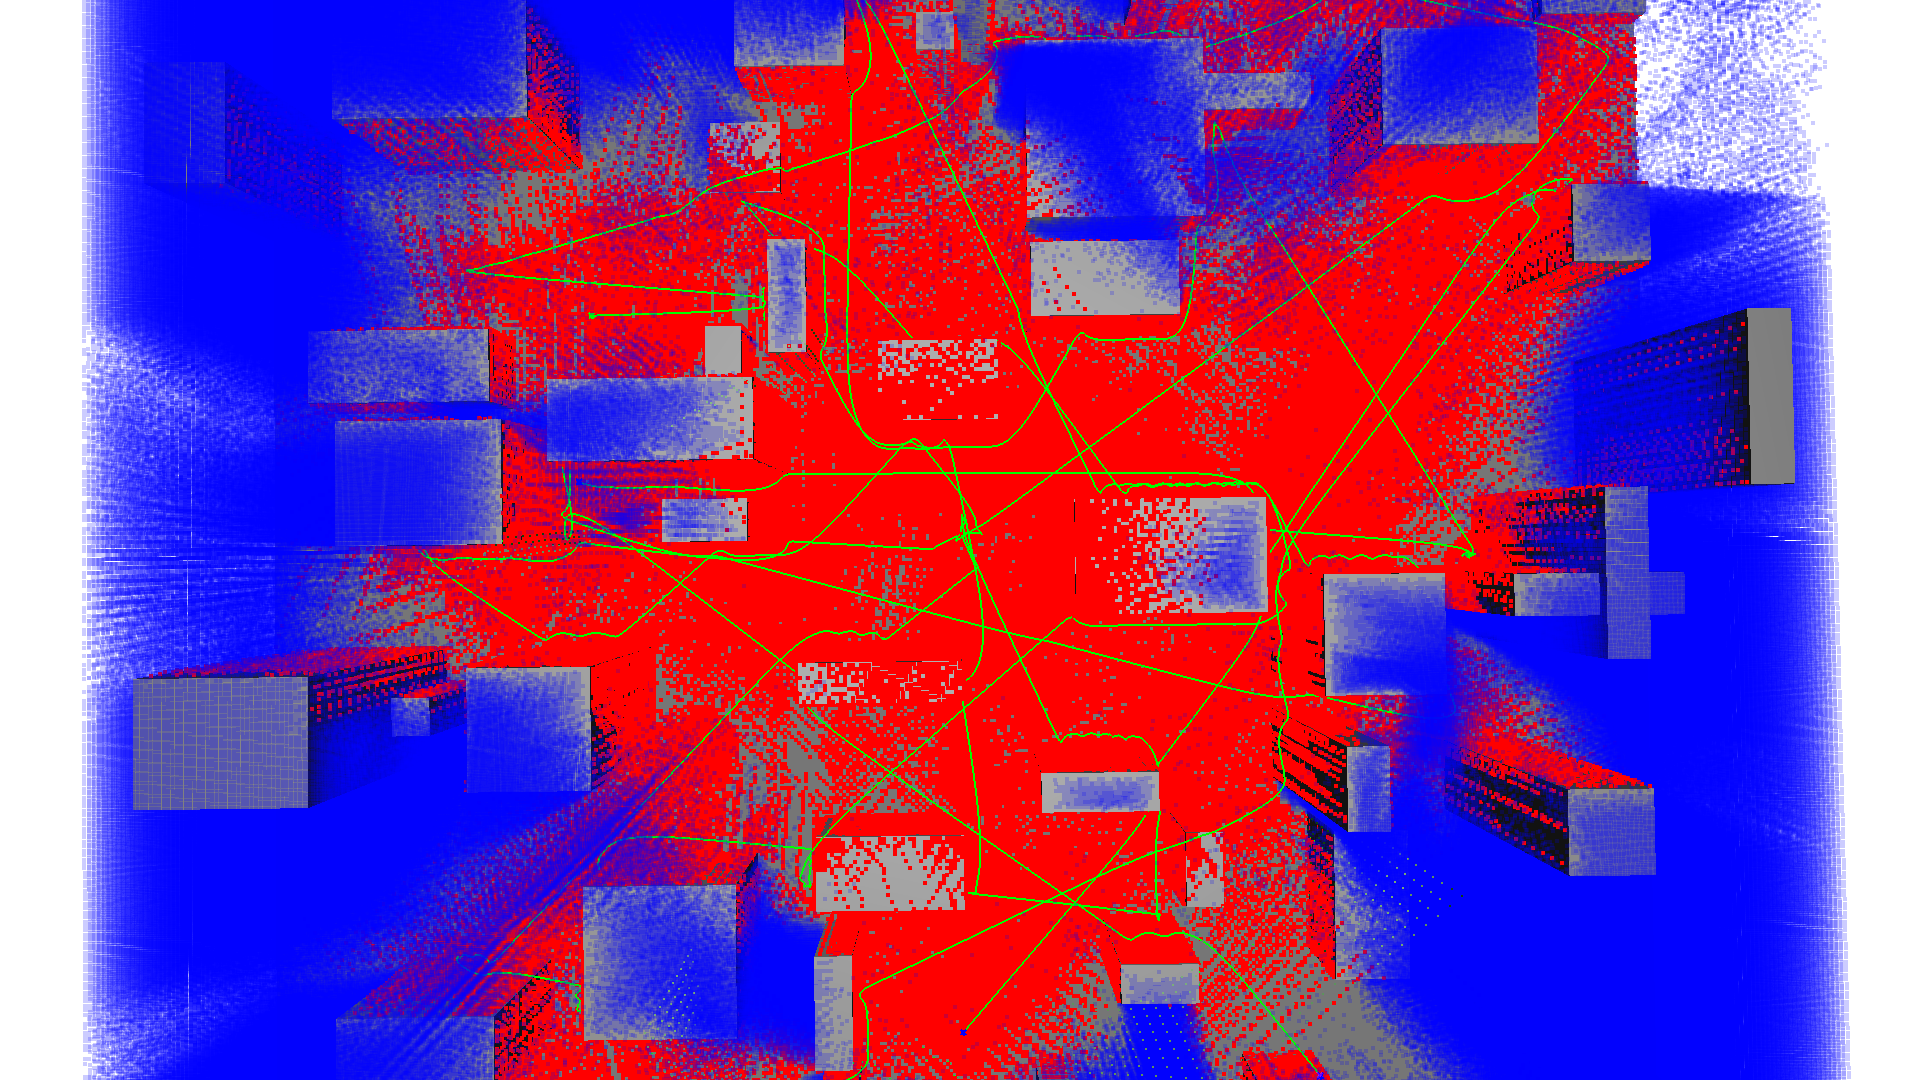
\includegraphics[width=\linewidth]{pa4.png}

Для реализации графической части был подготовлен код, выполняющий следующие функции:

\begin{mintemize}
\item Работа с оконной системой (\verb|SDL|)
\item Работа с 3D графикой (\verb|OpenGL|)
\end{mintemize}

\textbf{Работа с оконной системой}

Для работы с окнами была использована библиотека \verb|SDL| версии 2.0.
Так же эта библиотека позволяет получать события мыши и клавиатуры,
инициализировать контекст выполнения для \verb|OpenGL|.

Основные классы и структуры, используемые в ПМО:
\begin{mintemize}
\item \verb|DesApp| -- хранитель окон, распределяет события между окнами, реализует
    инициализацию контекста \verb|OpenGL|
\item \verb|DesWindow| -- окно, содержит набор сигналов, для реакции на события окна
    (изменение размера, сворачивание и тд), событий мыши, событий клавиатуры
\item \verb|MouseEvent| -- событие мыши
\item \verb|KeyboardEvent| -- событие нажатия клавиши
\end{mintemize}

Код можно найти в проекте \verb|DES|, который доступен по
\linebreak URL: \verb|https://github.com/dexset/des|.
Модуль \verb|des.app|.

\textbf{Работа с 3D графикой}

Библиотека для работы с 3D графикой \verb|OpenGL| имеет множество концепций для реализации
своего функционала. Перечислим использованные для работы ПМО:

\begin{mintemize}
\item \verb|vertex buffer object| -- буфер информации,
    хранимый на видеокарте, используемый для отрисовки
    (\verb|class GLBuffer|)
\item \verb|vertex array object| -- буфер параметров для
    группы \verb|vertex buffer object| (\verb|class GLVAO|)
\item \verb|shader program| -- программы, описывающие
    отображение буферов \linebreak (\verb|class ShaderProgram|)
\item \verb|texture| -- растровые изображения, хранящиеся
    в видеопамяти (\verb|class GLTexture|)
\item \verb|render buffer| -- растровое изображение, создаваемое
    исключительно для хранения результатов рендеринга
    (\verb|class GLRenderBuffer|)
\item \verb|frame buffer| -- набор растровых изображений,
    для хранения результатов рендеринга, отдельно цвет,
    глубина и тд (\verb|class GLFrameBuffer|)
\end{mintemize}

Каждый из этих классов является наследником от \verb|DesObject|
(\verb|des.util.arch|), который, в свою очередь, реализует интерфейс
\verb|ExternalMemoryManager|.

Модуль \verb|des.gl|.

Так же в модуле есть множество другого кода (проверка GL ошибок,
упрощённое использование объектов и тд).

\newpage
\subsubsection{Симуляция МБПЛА}

Симуляция работы МБПЛА выполнена в отдельной части программы,
связываемой с графической частью лишь необходимым для отрисовки
набором методов.

Некоторые концепции работы МБПЛА нашли не прямое отражение в ПМО.
Например карта местности на уровне кода не распределяется по юнитам,
а хранится в массиве, доступном всем юнитам. Это в первую очередь
связанно с быстродействием.

Симуляция работы МБПЛА проходит с фиксированным шагом интегрирования.

\newpage
\textbf{Модель карты местности}

Информация о местности представляется в виде трёхмерных сеток с фиксированными
высотой, шириной и глубиной. Каждый сектор это прямоугольная область пространства.
Информация, ассоциированная с каждым прямоугольным сектором, отличается для разных
карт. Разные карты могут иметь различное количество секторов, но пространственно
друг другу эквивалентны.

Различные типы карт содержат разную информацию:

\begin{mintemize}

\item Геометрическая

    \begin{mintemize}
    \item факт обследования
    \item наличие объекта
    \item количество замеров
    \item время последнего замера
    \end{mintemize}

\item Тепловая

    \begin{mintemize}
    \item факт обследования
    \item температура
    \item количество замеров
    \item время последнего замера
    \end{mintemize}

\item Радиокарта

    \begin{mintemize}
    \item факт обследования
    \item мощность внешнего радиосигнала по частотам
    \item количество замеров
    \item время последнего замера
    \end{mintemize}

\end{mintemize}

В ПМО реализован только первый тип карты: геометрическая. Это связанно с тем, что
реализация других типов карт не влияет по большому счёту на значительную часть
алгоритмов перемещения юнитов.

Реализация карты (информация, ассоциированная с пространственными секторами)
представляет собой 1-мерный массив, к которому можно обратиться с помощью трёх
индексов-координат.

Правила перевода индекса в координаты и обратно:

\nextverbatimspread{1}
\begin{verbatim}
    z = index / ( width * height )
    tmp = index % ( width * height )
    y = tmp / width
    x = tmp % width

    index = z * width * height + y * width + x
\end{verbatim}
\vspace{-0.5em}

где:

\verb|a / b| -- целочисленное деление \verb|a| на \verb|b|;

\verb|a % b| -- остаток от деления \verb|a| на \verb|b|;

\verb|index| -- индекс в одномерном массиве;

\verb|width| -- ширина поля;

\verb|height| -- высота поля;

\verb|x,y,z| -- координаты по ширине, высоте и глубине соответственно.

Также для карты имеется матрица трансформации координат из локальных (индексов)
в глобальные (метры).

При разрешении карты $400 \times 400 \times 50$ получаем $8 \cdot 10^6$ секторов.
Обработку таких объёмов данных было решено производить с помощью гетерогенных 
вычислений на GPU. Была использована технология \verb|OpenCL|. Это так же 
позволяет решить вопрос отображения данных через \verb|OpenGL|, так как
интероперабельность с графической системой использует zero-copy память -- 
физически это один участок памяти для буферов \verb|OpenCL| и \verb|OpenGL|.

\newpage
\textbf{Модель единицы массива}

Юнит в программе представлен как класс, реализующий интерфейс \verb|SpaceNode|.
Это позволяет удобно оперировать системами координат. \verb|SpaceNode| хранит
матрицу трансформации из связанно системы координат в местную, что упрощает
отрисовку юнита в интерфейсе. Каждый юнит имеет номер, это необходимо для
организации иерархических связей в начале работы.

Фазовый вектор юнита представлен в виде структуры, состоящей из двух векторов.

\nextverbatimspread{1}
\begin{verbatim}
struct PhVec
{
    vec3 pos;
    vec3 vel;

    mixin( BasicMathOp!"pos vel" );
}
\end{verbatim}

где: 

\verb|vec3 pos| -- положение юнита в пространстве

\verb|vec3 vel| -- скорость юнита в глобальной системе координат

\verb|mixin( BasicMathOp!"pos vel" )| -- реализация операций сложения,
вычитания, умножения и деления для структуры \verb|PhVec| 

Так же
у каждого юнита имеется набор различных параметров:

\nextverbatimspread{1}
\begin{verbatim}
\end{verbatim}


Примерный код функции $limit \left( \vec f \right)$:

\nextverbatimspread{1}
\begin{verbatim}
    vec3 limit( vec3 f )
    {
        if( f.xy.len > max_horisontal_force )
            f.xy = f.xy.e * max_horisontal_force;
        if( f.z > max_up_force ) f.z = max_up_force;
        if( f.z < min_up_force ) f.z = min_up_force;
        return f;
    }
\end{verbatim}

где:

\verb|f.xy| -- вектор, составленный из компонент вектора \verb|f|,

\verb|f.xy.len| -- длина вектора,

\verb|f.xy.e| -- единичный вектор.

Такой алгоритм обрезки максимальной тяги позволяет в горизонтальной плоскости двигаться к цели прямолинейно,
а выход на требуемую высоту происходит максимально быстро.

\newpage
\textbf{Модель измерителей и заполнение карты (!)}

Предполагается, что каждый юнит имеет возможность
оценить дальность в любом направлении, в нескольких точках одновременно с определённым 
угловым разрешением (карта глубин).

Каждый юнит получает информацю о мире с помощью датчика глубины в виде картинки,
где каждому пикселю соответствует измерение дальности в определённых угловых координатах. В работе не эмулировлись
дистрозийные искажения, поэтому для приведения карты глубин в точки в системе координат юнита достаточно 
матрицы перспективной трансформации, которая имеется у каждого юнита. Она также может меняться в процессе работы
системы при необходимости (изменение угла обзора, зум). Строится эта матрица так:

$$
M_{persp} = \left( \begin{array}{c c c c}
        \frac{1}{ R \cdot \tan( \frac{1}{2} A ) } & 0 & 0 & 0 \\
        0 & \frac{1}{ \tan( \frac{1}{2} A ) } & 0 & 0 \\
        0 & 0 & \frac{ z_{n} + z_{f} }{ z_{n}-z_{f} } & \frac{ 2 \cdot z_{n} \cdot z_{f} }{ z_{n} - z_{f} } \\
        0 & 0 & -1 & 0
\end{array} \right)
$$

где:

$R = \frac{w}{h}$ -- соотношение сторон изображения

$A$ -- угол обзора по вертикали

$z_{n}$ -- дальность от центра камеры до ближней плоскости отсечения

$z_{f}$ -- дальность от центра камеры до дальней плоскости отсечения

При трансформации точки с помощью перспективной матрицы координаты результирующей точки
получаются в диапазоне $x \in [-1,1]$, $y \in [-1,1]$, $z \in [0,1]$. Все точки, что выходят
за эти пределы, не отображаются. Для работы с четырёхменой матрицей необходимо использовать
однородные координаты.

Переход от однородных координат к декартовым: 

\verb|vec3 C = U.xyz / U.w|

Переход от декартовых к однородным:

\verb|vec4 U = vec4( C.xyz, 1 )|

где:

\verb|U| -- четырёхмерный вектор однородных координат,

\verb|C| -- трёхмерный вектор в декартовых координатах.

Процесс получение карты глубин реализован посредством \verb|OpenGL|. Для этого 
производится рендеринг мира в Frame Buffer, где для карты глубин выставлена текстура, 
которая потом копируется в буфер \verb|OpenCL|. Копирование из текстуры в буфер реализованно
из-за ограничений \verb|OpenCL 1.1|. Прямое использование изображений с глубиной добавленно
только в стандарте \verb|OpenCL 2.0|, вышедшем в 2013г. Драйвер видеокарты на рабочей машине
не поддерживал последний стандарт.

Точки имеют дополнительную информацию -- было ли что-либо найдено.
Это вычисляется с так: \verb|bool finded = depth[iy*w+ix] < 1.0f - 1e-6;|.
То есть, если значение глубины крайне близко к максимальному, можно считать, что
луч из камеры не наткнулся ни на один объект.

После получения точек в связанной системе координат они приводятся
сначала к мировой, затем к системе координат карты.
Так же приводится положение юнита (камеры) к системе координат карты.

Заполняется карта по следующему алгоритму:
\begin{mintemize}
    \item строится отрезок из точки камеры (А) к точке, полученной с датчика (Б)
    \item все сектора, которые находятся между А и Б помечаются как исследованные
    \item сектор, в котором находится точка с датчика помечается как заполненый,
        если в ней было что-то найдено.
\end{mintemize}
